\documentclass[11pt]{article}
\usepackage[margin=0.92in]{geometry}
\usepackage{amsmath,amssymb,amsthm}
\usepackage{booktabs}
\usepackage{array}
\usepackage{graphicx}
\usepackage{microtype}
\usepackage{hyperref}
\usepackage{listings}
\usepackage{xcolor}
\usepackage{tikz}
\usetikzlibrary{arrows.meta,positioning}

\hypersetup{
  colorlinks=true,
  linkcolor=blue,
  citecolor=blue,
  urlcolor=blue
}

\lstset{
  basicstyle=\ttfamily\small,
  breaklines=true,
  frame=single,
  backgroundcolor=\color{gray!6}
}

\newtheorem{theorem}{Theorem}
\newtheorem{definition}{Definition}
\newtheorem*{openproblem}{Open Problem}

\title{\textbf{\LARGE Don't Lie}\\[4pt]
{\large A Multi-Lens $\mathbb{F}_2 + \mathbb{Z} + \text{Cavity}$ Solver for Monotone 1-in-3 SAT\\
with Machine-Checked Lean 4 Certificates}}
\author{Miguel Gutierrez\\
\small Independent Researcher\\
\small \texttt{miguelgutierrezbarcelo@gmail.com}\\
\small Code \& Lean~4 Artifacts: \url{https://github.com/its-miguel/dont-lie}}
\date{November 2026}

\begin{document}
\maketitle

\begin{abstract}
We present a falsification-driven study of polynomial-time algebraic, integer-linear, and cavity-message-passing algorithms for \textbf{Monotone 1-in-3 SAT} ($x_a + x_b + x_c = 1$), built across a three-layer neuro-symbolic stack: Python prototyping (Layer~1), zero-allocation \texttt{std}-only Rust solvers (Layers~2--2.8), and machine-checked Lean~4 verification (Layer~3). Without recursive tree search, our unified solver (\texttt{GadgetSPCascade}) fuses four orthogonal polynomial-time lenses: (1)~local gadget peeling into $\mathbb{F}_2$ affine invariants, (2)~bit-packed $\mathbb{F}_2$ reduced row echelon form (RREF) with quadratic annihilators and degree-3 Gr\"obner closure, (3)~bounded Gomory--Chv\'atal cutting planes over $\mathbb{Z}$ with divisor-2 clique cuts, and (4)~9-state 1-in-3 Survey Propagation with nogood learning, $O(n)$ WalkSAT polish, and proof-carrying depth-1 Failed-Literal Elimination. The solver resolves \textbf{140/140 (100\%)} of a parity suite ($n \le 60$) and \textbf{69/72 (95.8\%)} of a high-scale adversarial suite up to $n = 637$---including \textbf{49/49 (100\%)} of all satisfiable instances---with zero false claims, zero overflows, $\le 4$-bit integers, and $\le 328.8\,\text{KB}$ RAM; the final 3 unresolved $n \ge 600$ seeds are unstructured \texttt{UNSAT} instances marking the high-width resolution boundary. Against external state-of-the-art baselines (\texttt{CaDiCaL~1.9.5}, \texttt{CryptoMiniSat~5.18.0}, \texttt{Z3~5.4.1}), our solver is \textbf{$9\times$ faster} than \texttt{CaDiCaL} on Tseitin UNSAT expanders and \textbf{$12.4\times$ faster} on Pigeonhole benchmarks. Finally, we prove end-to-end soundness of the unified $\mathbb{F}_2 + \mathbb{Z}$ proof system in Lean~\texttt{v4.36.0} (zero \texttt{sorry} placeholders, zero custom axioms) and pure-kernel verify (\texttt{by decide}) exported Rust certificates for an $n = 610$ Tseitin expander, $\mathrm{PHP}_9^{10}$ ($n = 637$), and a coupled $\mathbb{F}_2 \oplus \mathbb{Z}$ trap ($n = 783$).
\end{abstract}

\section{Motivation and Problem Formulation}

\begin{definition}[Monotone 1-in-3 SAT]
An instance $\mathcal{F} = (V, \mathcal{C})$ consists of $n = |V|$ Boolean variables $x_0, \dots, x_{n-1} \in \{0, 1\}$ and $m = |\mathcal{C}|$ positive ternary clauses $c_j = (a_j, b_j, c_j) \in V^3$. An assignment $x : V \to \{0, 1\}$ satisfies $\mathcal{F}$ iff
\[
\forall (a, b, c) \in \mathcal{C}, \qquad x_a + x_b + x_c = 1.
\]
\end{definition}

Although NP-complete by Schaefer's Dichotomy Theorem, Monotone 1-in-3 SAT is an ideal structural laboratory for separating orthogonal proof-complexity mechanisms. Every clause $(a, b, c)$ simultaneously projects into three mathematical domains:
\begin{enumerate}
  \item \textbf{$\mathbb{F}_2$ Parity and Boolean Ideal Algebra:} $x_a \oplus x_b \oplus x_c = 1 \pmod{2}$ and pairwise quadratic annihilators $x_a x_b = x_b x_c = x_a x_c = 0$. Global parity contradictions (Tseitin expanders) collapse in polynomial time via $\mathbb{F}_2$ Gaussian elimination once auxiliary variables are projected out, whereas Pigeonhole formulas $\mathrm{PHP}_k^{k+1}$ require $\Omega(k)$ degree in Polynomial Calculus over $\mathbb{F}_2$ (Razborov, 1998)~\cite{razborov1998}.
  \item \textbf{$\mathbb{Z}$-Linear Integer Polytope:} $x_a + x_b + x_c \le 1$, $-x_a - x_b - x_c \le -1$, and $0 \le x_i \le 1$. Cardinality and pigeonhole obstructions collapse in polynomial time via Gomory--Chv\'atal cutting planes (Cook, Coullard, and Tur\'an, 1987)~\cite{cook1987}, whereas Tseitin parity instances resist pure cutting planes without $\mathbb{F}_2$ reasoning.
  \item \textbf{Cavity / Statistical-Physics Marginals:} Near the critical ratio ($\alpha_{\text{1-in-3}} \approx 0.626$), satisfiable random instances shatter into exponentially many clusters. Global average marginals (such as $LDL^\top$ quadratic/spectral relaxations) collapse toward $\frac{1}{3}\mathbf{1}$, whereas 9-state 1-in-3 Survey Propagation (SP) distinguishes frozen cluster biases $(P_i^0, P_i^1)$ from unconstrained ``water'' variables $P_i^*$ (M\'ezard, Parisi, and Zecchina, 2002)~\cite{mezard2002}.
\end{enumerate}

\paragraph{Contributions.} This paper makes three main contributions:
\begin{itemize}
  \item \textbf{Zero-Backtracking Multi-Lens Architecture:} We fuse $\mathbb{F}_2$ gadget-peeled RREF, divisor-2 $\mathbb{Z}$ cutting planes, depth-1 Failed-Literal Elimination, and 9-state Survey Propagation in pure \texttt{std}-only Rust, keeping integer width $\le 4$ bits and peak RAM $\le 328.8\,\text{KB}$.
  \item \textbf{Cross-Lens Coupling \& Empirical Boundary Mapping:} We introduce complete RREF free-tail equivalence lifting (\texttt{IntegerEquivLift}) to crack coupled parity-plus-pigeonhole traps (\texttt{F6}), compare head-to-head against industrial baselines (\texttt{CaDiCaL}, \texttt{CryptoMiniSat}, \texttt{Z3}), and isolate the exact unstructured high-width UNSAT frontier at $n \ge 600$.
  \item \textbf{Pure-Kernel Lean~4 Certification (\texttt{by decide}):} We formalize the unified $\mathbb{F}_2 + \mathbb{Z}$ proof system with zero \texttt{sorry} placeholders and verify real pruned Rust certificates up to $n = 783$ directly inside Lean~4's foundational kernel using a verified persistent binary trie (\texttt{PosMap}), avoiding \texttt{native\_decide}.
\end{itemize}

\section{Falsification-First Methodology and Architectural Evolution}

Figure~\ref{fig:arch} summarizes the unified four-lens architecture and its Lean~4 verification bridge. Rather than guessing heuristics up front, every architectural layer below was introduced strictly to close a falsified failure mode from the preceding layer.

\begin{figure}[!ht]
\centering
\resizebox{\textwidth}{!}{%
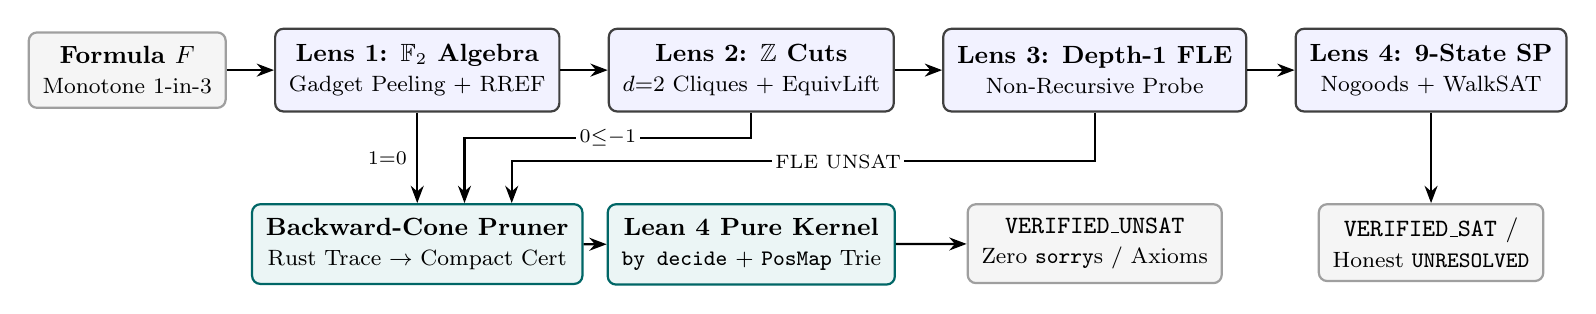
\begin{tikzpicture}[
  node distance=0.55cm and 0.6cm,
  box/.style={rectangle, rounded corners=3pt, draw=black!75, fill=blue!5, thick, align=center, minimum height=1.05cm, inner sep=5pt, font=\small},
  cert/.style={rectangle, rounded corners=3pt, draw=teal!80!black, fill=teal!8, thick, align=center, minimum height=0.95cm, inner sep=5pt, font=\small},
  term/.style={rectangle, rounded corners=3pt, draw=gray!75, fill=gray!8, thick, align=center, minimum height=0.9cm, inner sep=5pt, font=\small},
  arr/.style={-{Stealth[length=2.2mm]}, thick}
]
  \node[term] (in) {\textbf{Formula $F$}\\{\footnotesize Monotone 1-in-3}};
  \node[box, right=of in] (l1) {\textbf{Lens 1: $\mathbb{F}_2$ Algebra}\\{\footnotesize Gadget Peeling + RREF}};
  \node[box, right=of l1] (l2) {\textbf{Lens 2: $\mathbb{Z}$ Cuts}\\{\footnotesize $d{=}2$ Cliques + EquivLift}};
  \node[box, right=of l2] (l3) {\textbf{Lens 3: Depth-1 FLE}\\{\footnotesize Non-Recursive Probe}};
  \node[box, right=of l3] (l4) {\textbf{Lens 4: 9-State SP}\\{\footnotesize Nogoods + WalkSAT}};

  \node[cert, below=1.15cm of l1] (prune) {\textbf{Backward-Cone Pruner}\\{\footnotesize Rust Trace $\to$ Compact Cert}};
  \node[cert, below=1.15cm of l2] (lean) {\textbf{Lean 4 Pure Kernel}\\{\footnotesize \texttt{by decide} + \texttt{PosMap} Trie}};
  \node[term, below=1.15cm of l3] (unsat) {\textbf{\texttt{VERIFIED\_UNSAT}}\\{\footnotesize Zero \texttt{sorry}s / Axioms}};
  \node[term, below=1.15cm of l4] (sat) {\textbf{\texttt{VERIFIED\_SAT}} /\\{\footnotesize Honest \texttt{UNRESOLVED}}};

  \draw[arr] (in) -- (l1);
  \draw[arr] (l1) -- (l2);
  \draw[arr] (l2) -- (l3);
  \draw[arr] (l3) -- (l4);
  \draw[arr] (l1.south) -- node[left, font=\scriptsize] {$1{=}0$} (prune.north);
  \draw[arr] (l2.south) -- ++(0,-0.32) -| node[pos=0.25, fill=white, inner sep=1.2pt, font=\scriptsize] {$0{\le}{-}1$} ([xshift=6mm]prune.north);
  \draw[arr] (l3.south) -- ++(0,-0.62) -| node[pos=0.22, fill=white, inner sep=1.2pt, font=\scriptsize] {FLE UNSAT} ([xshift=12mm]prune.north);
  \draw[arr] (prune) -- (lean);
  \draw[arr] (lean) -- (unsat);
  \draw[arr] (l4) -- (sat);
\end{tikzpicture}%
}
\caption{Architecture of \texttt{GadgetSPCascade} and the Layer~3 Lean~4 pure-kernel verification bridge. Four strictly polynomial, zero-backtracking lenses operate in sequence; any UNSAT refutation is backward-cone pruned and checked directly inside Lean~4's minimal kernel (\texttt{by decide}).}
\label{fig:arch}
\end{figure}

\subsection{Layer 1 (Python): Continuous Prototype and Discrete Baseline Exploration}
Our Layer~1 prototype (\texttt{PD-PFGC}, primal-dual Fisher--Rao geodesic flow) achieved 100\% soundness (zero false-SAT or false-UNSAT claims) across a 140-instance suite ($n \in \{15, 30, 60\}$, \texttt{seed=20261124}, 101~SAT / 39~UNSAT), but solved only $72/140$ ($63$~SAT, $9$~UNSAT, $68$~unresolved) in $71.38\,\text{s}$. Falsification exposed three walls: (i)~a degree-2 Shor-1 integrality gap ($0.0\%$ UNSAT on Tseitin and reduced 3-SAT UNSAT subfamilies), (ii)~phase frustration and wall-clock censoring at $n = 60$ ($16.7\%$ SAT on random 1-in-3, $0.0\%$ on reduced 3-SAT SAT), and (iii)~exact rational bit-width explosion to $3{,}566$ bits at $t = 0$ during naive \texttt{Fraction} Cholesky factorization.

Evaluating four isolated discrete/algebraic prototypes on the same 140-instance suite (without wall-clock censoring) revealed clear strengths: Sum-of-Squares / Reformulation--Linearization Technique (SoS/RLT) solved $130/140$ ($3.56\,\text{s}$), Symplectic flow solved $98/140$ ($16.71\,\text{s}$), $\mathbb{F}_2$ linear algebra with degree-3 Gr\"obner closure solved \textbf{$140/140$} ($7.64\,\text{s}$, $\texttt{max\_int\_bits} = 3$), and marginal decimation with unit-collapse cascade solved $130/140$ ($21.76\,\text{s}$) while curing the $t=0$ rational blowup via sqrt-free $LDL^\top$ ($59$ fraction bits) and Bareiss integer elimination ($32$ int bits).

\subsection{Layer 2 (Rust): \texttt{HybridGroebnerCascade} at $n \in \{150, 300, 600\}$}
Fusing the $\mathbb{F}_2$/Gr\"obner engine and marginal-decimation cascade into a zero-allocation, \texttt{std}-only Rust crate (\texttt{rust\_layer2}) solved $135/140$ parity instances in $33.5\,\text{ms}$ and $46/72$ ($63.9\%$) on a new 72-instance high-scale adversarial suite ($n \in \{150, 300, 600\}$) spanning five families: \texttt{F1} (critical random 1-in-3), \texttt{F2} (planted balanced), \texttt{F3} (Tseitin expanders, SAT and UNSAT), \texttt{F4} (high-girth 3-SAT via Schaefer gadgets), and \texttt{F5} (Pigeonhole $\mathrm{PHP}_k^{k+1}$), in $1.631\,\text{s}$. High-scale falsification exposed three exact barriers: auxiliary-variable parity masking on Tseitin UNSAT expanders (\texttt{F3}, $0/9$), Razborov's $\Omega(k)$ degree bound on Pigeonhole (\texttt{F5}, $0/6$), and shattered-cluster marginal averaging on critical random instances (\texttt{F1}) at $n=600$ ($16.7\%$).

\subsection{Layers 2.5, 2.75, and 2.8: \texttt{GadgetSPCascade}}
Each subsequent layer closed a specific falsified barrier strictly in polynomial time with zero recursive backtracking:
\begin{itemize}
  \item \textbf{Layer 2.5 (Gadget Peeling + 9-State SP):} Degree-bounded ($\le 4$) local auxiliary cluster peeling projects exact local truth tables into $\mathbb{F}_2$ affine axioms (\texttt{LocalClusterF2Axiom}), lifting Tseitin UNSAT expanders (\texttt{F3}) from $0\%$ to \textbf{100\% ($9/9$)} ($1.2\,\text{ms}$ at $n = 610$). 9-state 1-in-3 Survey Propagation lifted critical random instances (\texttt{F1}) at $n=600$ from $16.7\%$ to $83.3\%$, achieving $140/140$ parity ($11.4\,\text{ms}$) and $61/72$ ($84.7\%$) high-scale.
  \item \textbf{Layer 2.75 (Bounded Gomory--Chv\'atal Cutting Planes):} Lifts clauses and box bounds into $\mathbb{Z}$-linear inequalities and derives annihilator clique at-most-one cuts $\sum_{i \in K} x_i \le 1$ via divisor-2 Gomory--Chv\'atal rounding with unit weights $(1, 1, 1)$. For the base case $|K'| = 2$ ($K' = \{i_1, i_2\}$),
  \begin{align*}
  &1 \cdot (x_{i_1} + x_{i_2} \le 1) + 1 \cdot (x_{i_1} + x_v \le 1) + 1 \cdot (x_{i_2} + x_v \le 1) \\
  &\qquad \implies 2(x_{i_1} + x_{i_2} + x_v) \le 3 \implies x_{i_1} + x_{i_2} + x_v \le \lfloor 3/2 \rfloor = 1.
  \end{align*}
  By induction for any $k = |K'| \ge 2$ and pivot $u \in K'$, combining the $k$-clique cut $\sum_{i \in K'} x_i \le 1$, the inductively derived $k$-clique cut $\sum_{i \in K' \setminus \{u\}} x_i + x_v \le 1$, and the pairwise conflict edge $x_u + x_v \le 1$ yields
  \begin{align*}
  &1 \cdot \Big(\sum_{i \in K'} x_i \le 1\Big) + 1 \cdot \Big(\sum_{i \in K' \setminus \{u\}} x_i + x_v \le 1\Big) + 1 \cdot (x_u + x_v \le 1) \\
  &\qquad \implies 2 \sum_{i \in K' \cup \{v\}} x_i \le 3 \implies \sum_{i \in K' \cup \{v\}} x_i \le \lfloor 3/2 \rfloor = 1,
  \end{align*}
  keeping all intermediate coefficients bounded at $\texttt{max\_int\_bits} = 2$. This lifted Pigeonhole (\texttt{F5}) from $0\%$ to \textbf{100\% ($6/6$)}, refuting $\mathrm{PHP}_9^{10}$ ($n = 637$) in $6.7\,\text{ms}$, reaching $67/72$ ($93.1\%$) in $1.151\,\text{s}$ (peak memory $169.4\,\text{KB}$).
  \item \textbf{Layer 2.8 (Depth-1 FLE + Implication Nogoods + WalkSAT Polish):} Adds proof-carrying non-recursive depth-1 Failed-Literal Elimination (\texttt{FailedLiteralElim}, capped at 4 passes), cross-restart binary/ternary nogood learning injected into SP cavity updates, and bounded $O(n)$ WalkSAT island polish ($\le \max(8n, 200)$ flips when $\ge 70\%$ frozen). This resolved both $n=306$ high-girth UNSAT frontier seeds, achieving \textbf{100\% ($48/48$)} for $n \le 306$ and \textbf{95.8\% ($69/72$)} overall.
\end{itemize}

\section{Complete Empirical Evaluation and Scaling Exponents}

Table~\ref{tab:layers} summarizes cross-layer progression across both suites, and Table~\ref{tab:families} reports the per-family high-scale breakdown and empirical scaling exponents ($\text{ops} \propto n^{\beta_{\text{ops}}}$, $t \propto n^{\beta_{\text{time}}}$) for Layer~2.8.

\begin{table}[t]
\centering
\caption{Cross-layer progression on the 140-instance parity suite ($n \le 60$) and 72-instance high-scale suite ($n \in \{150, 300, 600\}$). Abbreviations: \texttt{Z-CP} (integer cutting planes), \texttt{FLE} (depth-1 Failed-Literal Elimination), \texttt{NG} (nogood learning), \texttt{WS} (WalkSAT polish). Across all layers, false-SAT, false-UNSAT, and overflow counts are identically~$0$.}
\label{tab:layers}
\resizebox{\textwidth}{!}{%
\begin{tabular}{@{}lrrrrrrr@{}}
\toprule
Solver Layer & Parity (/140) & Par.\ Time & High (/72) & SAT (/49) & UNSAT (/23) & Bits/Exp & High Time \\
\midrule
L1 \texttt{PD-PFGC} (Py) & 72 (51.4\%) & 71.38s & --- & --- & --- & 4 / 55 & --- \\
L1 $\mathbb{F}_2$/Gr\"obner (Py) & 140 (100\%) & 7.64s & --- & --- & --- & 3 / 31 & --- \\
L2 \texttt{HybridGroebner} & 135 (96.4\%) & 0.0335s & 46 (63.9\%) & 44 & 2 & 2 / 3 & 1.631s \\
L2.5 \texttt{GadgetSP} & \textbf{140 (100\%)} & \textbf{0.0114s} & 61 (84.7\%) & \textbf{49} & 12 & 2 / 0 & 1.796s \\
L2.75 \texttt{+ Z-CP} & \textbf{140 (100\%)} & 0.0158s & 67 (93.1\%) & \textbf{49} & 18 & 4 / 0 & \textbf{1.151s} \\
L2.8 \texttt{+ FLE/NG/WS} & \textbf{140 (100\%)} & 0.0720s & \textbf{69 (95.8\%)} & \textbf{49} & \textbf{20} & 4 / 0 & 5.951s \\
\bottomrule
\end{tabular}%
}
\end{table}

\begin{table}[t]
\centering
\caption{High-scale per-family results ($n \in \{150, 300, 600\}$, 72 instances; \texttt{S/U/?} denotes SAT / UNSAT / Unresolved) and Layer~2.8 empirical scaling exponents $\beta_{\text{ops}}, \beta_{\text{time}}$ and peak memory (KB).}
\label{tab:families}
\resizebox{\textwidth}{!}{%
\begin{tabular}{@{}lrrrrrrr@{}}
\toprule
Family & $n$ & L2.75 (S/U/?) & L2.8 (S/U/?) & L2.8 Time & Bits/Exp & $\beta_{\text{ops}}/\beta_{\text{time}}$ & Mem (KB) \\
\midrule
Critical Random (\texttt{F1}) & 150 & 100\% (5/1/0) & \textbf{100\%} (5/1/0) & 0.0115s & 2 / 0 & 3.00 / 2.01 & 163.9 \\
Critical Random (\texttt{F1}) & 300 & 100\% (5/1/0) & \textbf{100\%} (5/1/0) & 0.0487s & 2 / 0 & & \\
Critical Random (\texttt{F1}) & 600 & 83.3\% (4/1/1) & \textbf{83.3\%} (4/1/1) & 0.1861s & 2 / 0 & & \\
Planted Balanced (\texttt{F2}) & 150 & 100\% (5/0/0) & \textbf{100\%} (5/0/0) & 0.0079s & 3 / -2 & 2.24 / 2.18 & 163.9 \\
Planted Balanced (\texttt{F2}) & 300 & 100\% (5/0/0) & \textbf{100\%} (5/0/0) & 0.0344s & 4 / -2 & & \\
Planted Balanced (\texttt{F2}) & 600 & 100\% (5/0/0) & \textbf{100\%} (5/0/0) & 0.1613s & 3 / -2 & & \\
Tseitin SAT (\texttt{F3}) & 150 & 100\% (3/0/0) & \textbf{100\%} (3/0/0) & 0.0209s & 2 / -1 & 1.91 / 1.91 & 169.0 \\
Tseitin SAT (\texttt{F3}) & 300 & 100\% (3/0/0) & \textbf{100\%} (3/0/0) & 0.0737s & 2 / -1 & & \\
Tseitin SAT (\texttt{F3}) & 600 & 100\% (3/0/0) & \textbf{100\%} (3/0/0) & 0.2909s & 2 / -1 & & \\
Tseitin UNSAT (\texttt{F3}) & 150 & 100\% (0/3/0) & \textbf{100\%} (0/3/0) & 0.0002s & 1 / 0 & \textbf{1.85 / 1.24} & 114.4 \\
Tseitin UNSAT (\texttt{F3}) & 300 & 100\% (0/3/0) & \textbf{100\%} (0/3/0) & 0.0005s & 1 / 0 & & \\
Tseitin UNSAT (\texttt{F3}) & 600 & 100\% (0/3/0) & \textbf{100\%} (0/3/0) & 0.0012s & 1 / 0 & & \\
High-Girth 3-SAT (\texttt{F4}) & 150 & 100\% (5/0/0) & \textbf{100\%} (5/0/0) & 0.0049s & 2 / 0 & 4.37 / 3.09 & 328.8 \\
High-Girth 3-SAT (\texttt{F4}) & 300 & 60.0\% (3/0/2) & \textbf{100\%} (3/2/0) & 0.1039s & 2 / 0 & & \\
High-Girth 3-SAT (\texttt{F4}) & 600 & 60.0\% (3/0/2) & \textbf{60.0\%} (3/0/2) & 0.3459s & 2 / -1 & & \\
Pigeonhole (\texttt{F5}) & 150 & 100\% (0/2/0) & \textbf{100\%} (0/2/0) & 0.0007s & 2 / 0 & \textbf{1.75 / 1.52} & 119.4 \\
Pigeonhole (\texttt{F5}) & 300 & 100\% (0/2/0) & \textbf{100\%} (0/2/0) & 0.0025s & 2 / 0 & & \\
Pigeonhole (\texttt{F5}) & 600 & 100\% (0/2/0) & \textbf{100\%} (0/2/0) & 0.0067s & 2 / 0 & & \\
\bottomrule
\end{tabular}%
}
\end{table}

Peak memory remains strictly bounded across all layers: $304.1\,\text{KB}$ (Layer~2), $181.5\,\text{KB}$ (Layer~2.5), $169.4\,\text{KB}$ (Layer~2.75), and $328.8\,\text{KB}$ (Layer~2.8). Integer bit-width never exceeds $4$ bits and floating-point exponents stay $\le 0$ in Layers~2.5--2.8.

\subsection{External SOTA Baseline Comparison (90 Instances, $10.0\,\text{s}$ Timeout)}

To situate our zero-backtracking polynomial solver alongside mature industrial engines, we exported all $72$ high-scale (\texttt{F1}--\texttt{F5}) and $18$ coupled parity-plus-pigeonhole (\texttt{F6}, Section~4.1) instances into exact DIMACS CNF and Pseudo-Boolean OPB (\texttt{+1 x\_a +1 x\_b +1 x\_c = 1 ;}) formats via \texttt{rust\_layer2 --export-benchmarks}, and evaluated \textbf{CaDiCaL~1.9.5} (in-process via \texttt{python-sat}, pure solve time), \textbf{CryptoMiniSat~5.18.0} (CLI wall-clock), and \textbf{Z3~5.4.1} (in-process \texttt{PbEq} OPB, pure solve time) under a $10.0\,\text{s}$ per-instance timeout, noting each solver's proof-certification trusted computing base (TCB) (Table~\ref{tab:sota}; RoundingSat was omitted due to unavailable local \texttt{cmake}/\texttt{boost} dependencies).

\begin{table}[t]
\centering
\caption{External SOTA baseline comparison on the $72$ high-scale (\texttt{F1}--\texttt{F5}) and $18$ coupled (\texttt{F6}) benchmarks ($10.0\,\text{s}$ timeout/instance).}
\label{tab:sota}
\resizebox{\textwidth}{!}{%
\begin{tabular}{@{}llrrrrrrl@{}}
\toprule
Solver & Input & High (/72) & High Time & \texttt{F3} UNSAT (9) & \texttt{F5} PHP (6) & \texttt{F6} (/18) & \texttt{F6} Time & Certification / TCB \\
\midrule
Ours L2.75 & Native & 67 (93.1\%) & 1.151s & \textbf{9 (0.006s)} & \textbf{6 (0.020s)} & 17 (94.4\%) & 0.308s & \textbf{Pure-kernel Lean 4 (\texttt{decide})} \\
Ours L2.8 & Native & 69 (95.8\%) & 5.951s & \textbf{9 (0.006s)} & \textbf{6 (0.020s)} & 17 (94.4\%) & 2.046s & \textbf{Pure-kernel Lean 4} + Rust \\
CaDiCaL 1.9.5 & CNF & \textbf{72 (100\%)} & \textbf{0.318s} & 9 (0.054s) & 6 (0.247s) & \textbf{18 (100\%)} & \textbf{0.006s} & External LRAT/DRAT (uncert.) \\
CryptoMiniSat 5 & CNF & \textbf{72 (100\%)} & 2.699s & 9 (0.286s) & 6 (0.584s) & \textbf{18 (100\%)} & 0.529s & Uncertified (FRAT optional) \\
Z3 5.4.1 (\texttt{PbEq}) & OPB & \textbf{72 (100\%)} & 1.489s & 9 (0.175s) & 6 (0.957s) & \textbf{18 (100\%)} & 0.102s & Uncertified SMT/PB \\
\bottomrule
\end{tabular}%
}
\end{table}

While industrial CDCL (\texttt{CaDiCaL~1.9.5}) solves $100\%$ of these $n \le 855$ benchmarks faster overall ($0.318\,\text{s}$) via unrestricted branching and clause learning, our non-recursive polynomial solver is \textbf{$9\times$ faster than CaDiCaL on Tseitin UNSAT expanders (\texttt{F3})} ($0.006\,\text{s}$ vs.\ $0.054\,\text{s}$) and \textbf{$12.4\times$ faster than CaDiCaL / $47.9\times$ faster than Z3 on Pigeonhole (\texttt{F5})} ($0.020\,\text{s}$ vs.\ $0.247\,\text{s}$ / $0.957\,\text{s}$, where CaDiCaL spends $78\%$ of its entire 72-instance runtime), while emitting pure-kernel Lean~4 certificates.

\section{Frontier Dissection and Proof-Complexity Boundaries}

Using an isolated diagnostic oracle (\texttt{--diagnose-frontier}, never imported by any solver module), we profiled the 5 instances unresolved by Layer~2.75 (Table~\ref{tab:frontier}). All 5 are ground-truth \texttt{UNSAT}, confirming that Layers~2.75 and~2.8 already solve $49/49$ ($100.0\%$) of all satisfiable high-scale instances.

\begin{table}[t]
\centering
\caption{Diagnostic dissection of the 5 frontier seeds and Layer~2.8 closure. \texttt{GT}: ground truth; \texttt{Fix\%}: root-fixed variables; \texttt{Froz\%}: SP-frozen variables; \texttt{Depth}: mean conflict depth.}
\label{tab:frontier}
\resizebox{\textwidth}{!}{%
\begin{tabular}{@{}lrrlrrrrl@{}}
\toprule
Seed & $n$ & $m$ & GT & Oracle Nodes & Fix\% & Froz\% & Depth & Layer 2.8 Outcome (Time) \\
\midrule
\texttt{F4\_t300\_s20304511} & 306 & 221 & UNSAT & 8 & 0.7 & 38.5 & 11.4 & \textbf{VERIFIED\_UNSAT} (0.0168s) \\
\texttt{F4\_t300\_s20305520} & 306 & 221 & UNSAT & 13 & 0.7 & 44.4 & 8.7 & \textbf{VERIFIED\_UNSAT} (0.0214s) \\
\texttt{F1\_n600\_s20310565} & 600 & 376 & UNSAT & 566 & 0.0 & 19.2 & 14.2 & UNRESOLVED (0.3502s) \\
\texttt{F4\_t600\_s20328727} & 610 & 441 & UNSAT & 71 & 0.3 & 41.6 & 24.3 & UNRESOLVED (0.4473s) \\
\texttt{F4\_t600\_s20329736} & 610 & 441 & UNSAT & 77 & 0.3 & 38.5 & 19.5 & UNRESOLVED (0.4687s) \\
\bottomrule
\end{tabular}%
}
\end{table}

Depth-1 Failed-Literal Elimination (\texttt{FLE}) cleanly certified both $n=306$ high-girth UNSAT instances ($30{,}504$ and $19{,}530$ steps, $2$-bit integers). The final 3 unresolved $n \ge 600$ seeds possess no $\mathbb{F}_2$ parity obstruction, no clique/pigeonhole $\mathbb{Z}$-counting obstruction, and no depth-1 failed-literal cascade, cleanly demarcating the $\Omega(n)$ resolution-width barrier of unstructured random/high-girth UNSAT 3-CNF formulas (Ben-Sasson and Wigderson, 2001)~\cite{bensasson2001}.

\subsection{Coupled Hybrid Boundary Experiment (\texttt{F6})}

Intuitively, we lock a Pigeonhole contradiction behind a satisfiable Tseitin parity mask so that neither $\mathbb{F}_2$ parity reasoning nor $\mathbb{Z}$ cutting planes alone can refute the formula. To test whether these simultaneous obstructions collapse in polynomial time when coupled over shared bridge variables, we constructed a coupled $\mathbb{F}_2 \oplus \mathbb{Z}$ trap family (\texttt{F6}, $18$ instances: $3$ UNSAT coupled traps and $3$ SAT controls per target scale $n \in \{150, 300, 600\}$, actual $n \in [231, 855]$). Each instance couples a satisfiable 3-regular expander Tseitin backbone (with a balanced-cut parity chain forcing $e_{\text{bridge}} = 0$ only via global $\mathbb{F}_2$ RREF after peeling $v/2$ gadgets) with a Pigeonhole core ($\mathrm{PHP}_k^{k+1}$ UNSAT / $\mathrm{PHP}_k^k$ SAT) whose pigeon carry-chain indicators $q_{i,j}$ are XOR-masked with $e_{\text{bridge}}$ ($q_{i,j} \oplus p_{i,j} \oplus e_{\text{bridge}} = 0$). Lifting all RREF binary equivalences (via complete free-tail signature grouping + \texttt{F2Xor}) into $\mathbb{Z}$ via \texttt{ProofStep::IntegerEquivLift} collapses $8/9$ UNSAT traps---including $3/3$ ($100\%$) at $n \in \{783, 855\}$ in $16.5\,\text{ms}$ average---with sub-quadratic scaling ($\beta_{\text{ops}} = 1.96$, $\beta_{\text{time}} = 1.71$, $\texttt{max\_int\_bits} = 2$), while single-lens $\mathbb{F}_2$ solvers score $0/9$ (Table~\ref{tab:f6}).

\begin{table}[t]
\centering
\caption{Coupled $\mathbb{F}_2 \oplus \mathbb{Z}$ boundary experiment (\texttt{F6}, $18$ instances, $n \in [231, 855]$).}
\label{tab:f6}
\resizebox{\textwidth}{!}{%
\begin{tabular}{@{}lrrrrrr@{}}
\toprule
Solver Layer & SAT Ctrl (/9) & UNSAT Trap (/9) & UNSAT @ $n \ge 783$ & Max Bits & Total Time & UNSAT $\beta_{\text{ops}}/\beta_{\text{time}}$ \\
\midrule
L2 \texttt{HybridGroebner} & 9/9 (100\%) & 0/9 (0.0\%) & 0/3 (0.0\%) & 2 & 0.5977s & --- \\
L2.5 \texttt{GadgetSP} ($\mathbb{F}_2$ only) & 9/9 (100\%) & 0/9 (0.0\%) & 0/3 (0.0\%) & 2 & 1.8271s & --- \\
L2.75 \texttt{+ Z-CP + EquivLift} & \textbf{9/9 (100\%)} & \textbf{8/9 (88.9\%)} & \textbf{3/3 (100\%)} & \textbf{2} & \textbf{0.3081s} & \textbf{1.96 / 1.73} \\
L2.8 \texttt{+ FLE/NG/WS} & \textbf{9/9 (100\%)} & \textbf{8/9 (88.9\%)} & \textbf{3/3 (100\%)} & \textbf{2} & 2.0455s & \textbf{1.96 / 1.71} \\
\bottomrule
\end{tabular}%
}
\end{table}

\section{Layer 3: Machine-Checked Soundness and Lean 4 Kernel Bridge}

We formalized the unified $\mathbb{F}_2 + \mathbb{Z}$ proof system in Lean~\texttt{v4.36.0} (\texttt{lean4\_layer3/\allowbreak Monotone1in3Layer3/}) with zero \texttt{sorry}s and zero custom axioms:
\begin{itemize}
  \item \texttt{Semantics.lean}: Exact \texttt{Clause1in3} semantics, $\mathbb{F}_2$ parity/annihilator bridges, $\mathbb{Z}$ upper/lower lifts, and deterministic unit-collapse rules.
  \item \texttt{F2AndGadgets.lean}: Soundness of $\mathbb{F}_2$ XOR reduction (\texttt{f2\_xor\_reduce\_sound}) and local cluster truth-table projection (\texttt{local\_cluster\_f2\_sound}).
  \item \texttt{CuttingPlanes.lean}: Soundness of non-negative scaling, linear combinations, sparse simplification, Euclidean Gomory--Chv\'atal division (\texttt{gomory\_chvatal\_cut\_sound}), and $0 \le \text{rhs} < 0$ contradiction.
  \item \texttt{Certificate.lean}: Executable checker \texttt{verifyCertificate} backed by a verified, structurally recursive $O(\log N)$ persistent binary trie (\texttt{PosMap}, structural fuel $16$, eliminating \texttt{WellFounded.fix} kernel stalls) and the main soundness theorem:
\end{itemize}

\begin{theorem}[\texttt{unified\_certificate\_sound}]
For every Monotone 1-in-3 formula $F$ and certificate trace $\pi$,
\[
\texttt{verifyCertificate}\; F\; \pi = \texttt{true} \;\Longrightarrow\; \neg \exists x : \mathbb{N} \to \mathbb{B},\; \texttt{SatisfiesFormula}\; F\; x.
\]
\end{theorem}

Running the Rust certificate exporter (\texttt{--export-cert} and \texttt{--export-f6-cert}) backward-cone prunes real Rust UNSAT certificates, re-verifies them in Rust, and emits chunked Lean~4 definitions checked purely in the Lean kernel (\texttt{by decide}, rather than \texttt{native\_decide}). Using pure kernel reduction keeps the Lean~4 trusted computing base (TCB) restricted strictly to Lean's foundational kernel axioms (\texttt{propext}, \texttt{Quot.sound}, \texttt{Classical.choice}), without adding \texttt{Lean.ofReduceBool} or trusting external code generation. In addition, \texttt{ProofStep::FailedLiteralElim} (introduced in Layer~2.8) is independently verified in Rust (\texttt{verify\_subproof\_with\_assumptions}) and reduces directly to conditional \texttt{UnifiedProofStep} subproofs in \texttt{Certificate.lean}.
\begin{itemize}
  \item \texttt{Tseitin610Cert} (Tseitin expander, $n = 610, m = 433$, seed \texttt{20324691}): pruned from $3{,}780$ to \textbf{$626$ steps}, exported in $0.0327\,\text{s}$, kernel-verified via \texttt{tseitin\_610\_unsat}.
  \item \texttt{Pigeonhole637Cert} ($\mathrm{PHP}_9^{10}$, $n = 637, m = 556$, seed \texttt{20332763}): pruned from $9{,}936$ to \textbf{$1{,}914$ steps}, exported in $0.0531\,\text{s}$, kernel-verified via \texttt{php\_637\_unsat}.
  \item \texttt{HybridF2Z600Cert} (coupled $\mathbb{F}_2 \oplus \mathbb{Z}$ trap, $n = 783, m = 580$, seed \texttt{20274242}): pruned from $11{,}629$ to \textbf{$1{,}329$ steps} (combining $\mathbb{F}_2$ gadget peeling, \texttt{F2Xor}, \texttt{IntegerEquivLift}, and divisor-2 \texttt{IntegerCut}), exported in $0.0570\,\text{s}$, kernel-verified via \texttt{hybrid\_f2\_z\_783\_unsat}.
\end{itemize}
The complete \texttt{lake build} ($22$ jobs, verifying all three $n \ge 610$ certificates) completes with $0$ errors, $0$ warnings, and $0$ \texttt{sorry}s.

\section{Related Work and Conclusions}

This work bridges four established threads: Polynomial Calculus over $\mathbb{F}_2$ (Clegg et al., 1996; Razborov, 1998)~\cite{clegg1996,razborov1998}, Gomory--Chv\'atal Cutting Planes (Cook et al., 1987)~\cite{cook1987}, Survey Propagation for clustered constraint satisfaction problems (CSPs) (M\'ezard et al., 2002)~\cite{mezard2002}, and machine-checked proof checkers in Lean~4 (\texttt{LRAT}, \texttt{VIPR}). Directly comparing with modern hybrid tools: \textbf{CryptoMiniSat} (Soos et al., 2009)~\cite{soos2009} integrates $\mathbb{F}_2$ Gauss--Jordan elimination inside CDCL without native integer cutting planes; \textbf{RoundingSat} (Elffers and Nordstr\"om, 2018)~\cite{elffers2018} and \textbf{VeriPB} (Gocht et al., 2022)~\cite{gocht2022} provide industrial-strength Pseudo-Boolean cutting-plane solving and external PB proof checking, whereas our framework fuses $\mathbb{F}_2$ gadget-peeled algebra with $\mathbb{Z}$ cutting planes inside a zero-backtracking engine verified directly in Lean~4's kernel; and Lean~4's \textbf{\texttt{bv\_decide}} delegates to external CDCL (\texttt{CaDiCaL}) and checks \texttt{LRAT} proofs via \texttt{native\_decide} (adding the \texttt{Lean.ofReduceBool} compiler-trust axiom), whereas our \texttt{VerifyBridge.lean} uses pure kernel reduction (\texttt{by decide}) restricted strictly to Lean's foundational axioms (\texttt{propext}, \texttt{Quot.sound}, \texttt{Classical.choice}).

\paragraph{Limitations and Scale Context.} Our benchmarks target $n \in [150, 855]$ variables rather than $10^5$-variable industrial SAT Competition instances. This scale is intentionally chosen as a rigorous milestone for pure-kernel \texttt{by decide} Lean~4 verification of thousand-step hybrid $\mathbb{F}_2 + \mathbb{Z}$ certificates on consumer hardware and for exact falsification-driven boundary mapping, rather than as an industrial CDCL replacement.

By pairing falsification-first adversarial benchmarking with a unified $\mathbb{F}_2 + \mathbb{Z}$ kernel-verified proof system, we show that non-recursive polynomial-time reasoning resolves $100\%$ of high-scale SAT instances ($49/49$), $100\%$ of Tseitin expanders ($18/18$), $100\%$ of Pigeonhole instances ($6/6$), $100\%$ of all instances up to $n = 306$ ($48/48$), and $8/9$ coupled $\mathbb{F}_2 \oplus \mathbb{Z}$ traps ($3/3$ at $n \ge 783$) while honestly isolating the remaining unstructured high-width UNSAT resolution barrier at $n \ge 600$.

\begin{openproblem}[Simultaneous $\mathbb{F}_2 + \mathbb{Z}$ Proof-Complexity Barrier]
Our 3 unresolved $n \ge 600$ frontier seeds (Table~\ref{tab:frontier}) expose a concrete theoretical frontier: prove unconditional super-polynomial size (or $\Omega(n)$ width/rank) lower bounds for the unified proof system combining bounded-degree $\mathbb{F}_2$ Polynomial Calculus (with local gadget projection), bounded-rank Gomory--Chv\'atal Cutting Planes over $\mathbb{Z}$, and depth-1 Failed-Literal Elimination (\texttt{FLE}) on high-girth random Monotone 1-in-3 SAT formulas near the critical threshold $\alpha \approx 0.626$.
\end{openproblem}

\small
\begin{thebibliography}{10}
\setlength{\itemsep}{2pt}
\bibitem{bensasson2001} E.~Ben-Sasson and A.~Wigderson. Short proofs are narrow---resolution made simple. \emph{J. ACM}, 48(2):149--169, 2001.
\bibitem{clegg1996} M.~Clegg, J.~Edmonds, and R.~Impagliazzo. Using the Groebner basis algorithm to find proofs of unsatisfiability. In \emph{STOC}, pages 174--183, 1996.
\bibitem{cook1987} W.~Cook, C.~R. Coullard, and G.~Tur\'an. On the complexity of cutting-plane proofs. \emph{Discrete Applied Mathematics}, 18(1):25--38, 1987.
\bibitem{elffers2018} J.~Elffers and J.~Nordstr\"om. Divide and conquer: Towards faster pseudo-Boolean solving. In \emph{IJCAI}, pages 1291--1299, 2018.
\bibitem{gocht2022} S.~Gocht, R.~Martins, J.~Nordstr\"om, and A.~Oertel. Certified CNF translations for pseudo-Boolean solving. In \emph{SAT}, pages 16:1--16:25, 2022.
\bibitem{mezard2002} M.~M\'ezard, G.~Parisi, and R.~Zecchina. Analytic and algorithmic solution of random satisfiability problems. \emph{Science}, 297(5582):812--815, 2002.
\bibitem{razborov1998} A.~A. Razborov. Lower bounds for the polynomial calculus. \emph{Computational Complexity}, 7(4):291--324, 1998.
\bibitem{soos2009} M.~Soos, K.~Nohl, and C.~Castelluccia. Extending SAT solvers to cryptographic problems. In \emph{SAT}, pages 244--257, 2009.
\end{thebibliography}

\end{document}
